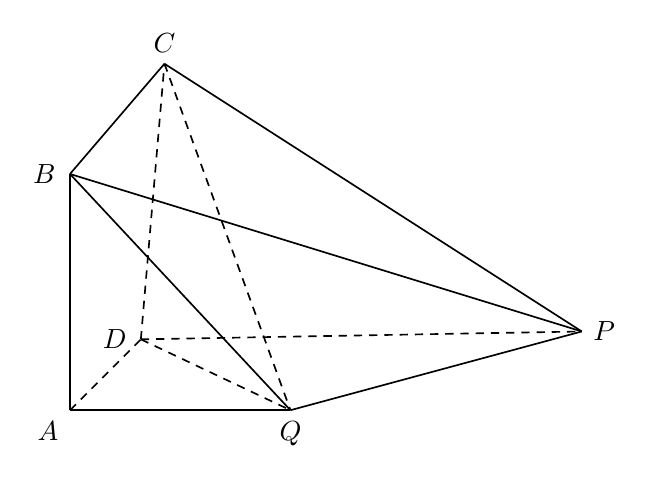
\begin{tikzpicture}[x=1cm,y=1cm,font=\normalsize]
\tikzset{edge/.style={draw=black,line width=.6pt,solid},hedge/.style={draw=black,line width=.6pt,dashed,dash pattern=on 3pt off 2.5pt},lbl/.style={font=\normalsize,inner sep=2pt}}
\coordinate (A) at (0,0);
\coordinate (Q) at (2.8,0);
\coordinate (B) at (0,3.0);
\coordinate (D) at (0.9,0.9);
\coordinate (P) at (6.5,1.0);
\coordinate (C) at (1.2,4.4);
\draw[edge] (A) -- (B);
\draw[edge] (A) -- (Q);
\draw[edge] (B) -- (C);
\draw[edge] (B) -- (Q);
\draw[edge] (B) -- (P);
\draw[edge] (C) -- (P);
\draw[edge] (P) -- (Q);
\draw[hedge] (A) -- (D);
\draw[hedge] (D) -- (C);
\draw[hedge] (D) -- (Q);
\draw[hedge] (C) -- (Q);
\draw[hedge] (D) -- (P);
\node[lbl,below left,xshift=-2pt,yshift=-2pt] at (A) {$A$};
\node[lbl,left,xshift=-3pt] at (B) {$B$};
\node[lbl,above,yshift=2pt] at (C) {$C$};
\node[lbl,left,xshift=-3pt] at (D) {$D$};
\node[lbl,below,yshift=-2pt] at (Q) {$Q$};
\node[lbl,right,xshift=2pt] at (P) {$P$};
\end{tikzpicture}
